\chapter{Web Application} \label{chap webApp}
\minitoc
Neste capítulo vamos expor alguns pormenores relacionados com a implementação do problema proposto.
Será explicada a maneira que encontramos para que seja seja cumprida a arquitectura que escolhemos e modelamos inicialmente.

\section{Criação de grupos, docentes e concorrentes}\label{sec gdc}
O sistema permite que qualquer utilizador não registado se registe como grupo ~\ref{img:signup}, e associe a si um ou mais concorrentes. Para efectuar o registo terá de preencher o nome do grupo/docente, um e-mail válido e uma password que tenha entre 6 a 40 caracteres.\\
Este login é utilizado por todo o grupo, para participar nos mais variados concursos.\\

\begin{figure}[H]
\begin{center}
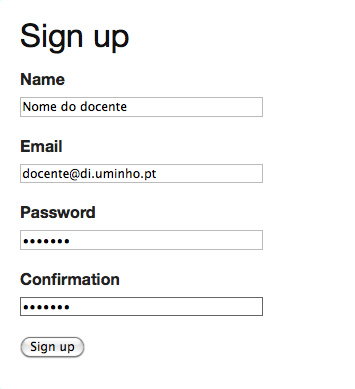
\includegraphics[width=0.45\textwidth]{Images/signup}
\caption{Página de registo}\label{img:signup}
\end{center}
\end{figure} 

Um concorrente é caracterizado por um nome, um número de aluno e um e-mail ~\ref{img:grupo}.

\begin{figure}[H]
\begin{center}
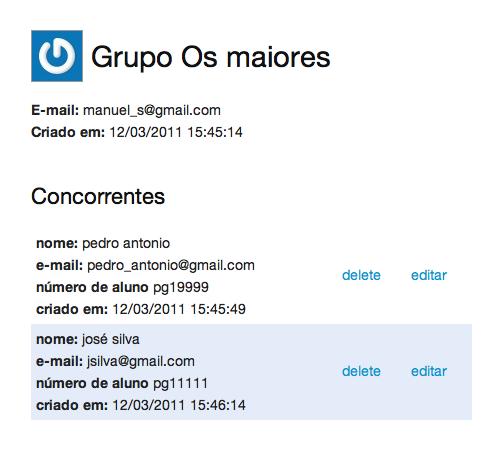
\includegraphics[scale = 0.6]{Images/grupo}
\caption{Dados de um grupo}\label{img:grupo}
\end{center}
\end{figure} 



As contas de docente só podem ser criados pelo administrador. Para simplificar o trabalho do administrador, o docente pode criar 
uma conta de grupo, à qual mais tarde será concedida privilégios de docente ~\ref{img:userToAdmin}.

\begin{figure}[H]
\begin{center}
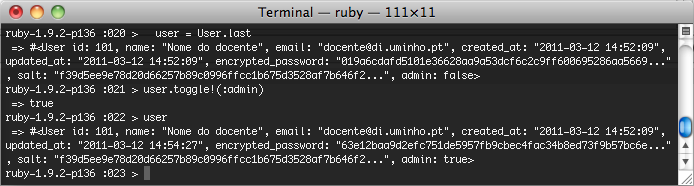
\includegraphics[scale=0.60]{Images/userToAdmin}
\caption{Comandos necessários para tornar um utilizador sem privilégios num docente.}\label{img:userToAdmin}
\end{center}
\end{figure} 

\section{Linguagens de programação}\label{sec lps}
O nosso sistema é multilingue, ou seja, é possível submeter código fonte em várias linguagens de programação diferentes, desde que 
a linguagem tenha sido correctamente configurada por um docente.
Cada linguagem é caracterizada por uma série de campos ~\ref{img:newLang}, os quais serão explicados de seguida:
\begin{itemize}
\item string de compilação: string que será executada quando se pretender compilar determinado código fonte. Esta string tem a
particularidade de no lugar em que é suposto conter o nome do ficheiro a compilar, contém \textit{\#\{file\}}.\\
Desta forma a string de compilação torna-se genérica, e independente do nome do ficheiro a compilar.
exemplo: gcc -O2 -Wall \#\{file\}

\item string simples de execução: string utilizada para executar quando o código fonte foi compilado pela string de compilação.\\
exemplo 1:\\ 
- string de compilação: gcc -O2 -Wall \#\{file\}\\
- string de execução respectiva: ./a.out\\
exemplo 2:\\
- string de compilação: gcc -O2 -Wall \#\{file\} -o exec\\
- string de execução respectiva: ./exec\\

\item string complexa de execução: a necessidade de uma segunda string de execução surgiu quando tentamos preparar o sistema para receber makefiles (inicialmente apenas para C). Nestes casos, o nome do executável gerado pela compilação não é conhecido à partida.
Desta forma é necessário analisar o makefile, e só depois executar, tendo em conta a informação que retiramos do makefile.\\
Assim, e para a linguagem C, a string complexa de execução seria:\\
- ./\#\{file\}\\
em que \#\{file\} representa o nome do executável.

\begin{figure}[H]
\begin{center}
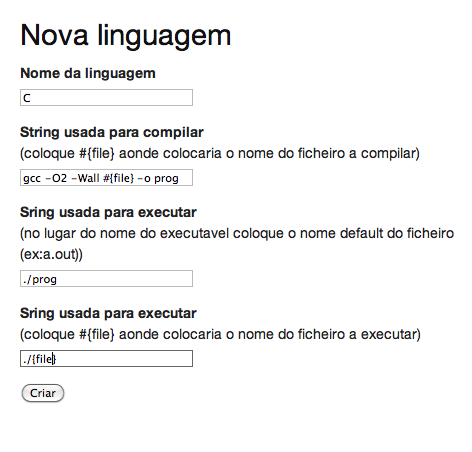
\includegraphics[scale=0.60]{Images/newLang}
\caption{Configuração de uma nova linguagem de programação no sistema}\label{img:newLang}
\end{center}
\end{figure} 

\end{itemize}

\section{Submissão de programas}\label{sec subm}
Sempre que acharem adequado, os grupos podem submeter os seus programas para serem avaliados. Para tal têm de escolher a linguagem de programação na qual resolveram o problema, de entre as disponíveis. E de seguida basta escolherem o ficheiro que pretendem submeter e carregar no botão de submissão.\\
No caso do administrador, pode ainda submeter tentativas no formato XML.

\begin{figure}[H]
\begin{center}
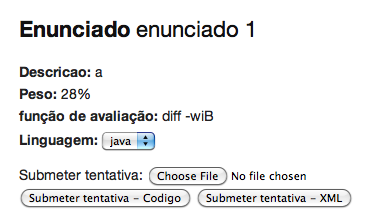
\includegraphics[scale=0.60]{Images/submissao}
\caption{Página de submissão de programas (vista de administrador)}\label{img:subm}
\end{center}
\end{figure} 

\section{Compilação}\label{sec comp}

Estando as linguagens de programação correctamente configuradas, a compilação torna-se bastante simples. Quando uma tentativa
é submetida no sistema, começamos por verificar se foi submetida apenas um ficheiro de código, ou um ficheiro comprimido.\\
Caso seja apenas um ficheiro, o sistema tenta compilar o código submetido, com a string de compilação da linguagem de programação em causa.\\
No caso de se tratar de um ficheiro comprimido, depois de o descomprimir, o sistema verifica se existe um makefile entre os ficheiros extraídos. Caso se verifique, é corrido o comando \textit{make}, e tenta retirar o nome do executável gerado, de modo a poder
ser usado na execução.

\section{Execução}\label{sec exec}
No fim da compilação, o sistema vai executar o programa uma vez para cada input. O processo de execução no caso de a compilação ter
sido feita à custa do makefile, é feita usando a string complexa de execução (sendo o nome do executável aquele que foi retirado do
makefile) . Se tal não tiver acontecido, é usada a string simples.\\
A execução pode ser abortada se ultrapassar o tempo máximo de execução, que é definido aquando da criação do enunciado em
questão. A título de demonstração, de seguida apresentamos a porção de código que "mata" o processo relativo à execução do programa,
caso ele demore mais de que o tempo máximo.

\begin{haskell}
    #thread que executa o a.out 
    out = "default";i=0
    exec = Thread.new do
      out = `#{execString} #{input}`
    end
    
    #thread que conta x segundos e dps termina a execucao do programa
    timer = Thread.new do
      sleep 5
      if exec.alive?
        Thread.kill(exec)
        i=1
        if params[:tentativa][:execStop] == false
          @erros += "Time out! Pelo menos a execucao de um dos inputs foi terminada por demorar demasiado tempo!"
        end
        params[:tentativa][:execStop] = true
      end
    end
    
    exec.join
    if timer.alive?
      Thread.kill(timer)
    end
    timer.join

\end{haskell}

\section{Guardar resultados}\label{sec res}
Para cada input do enunciado em questão, o programa é executado uma vez. O seu output é comparado com o output esperado e 
é guardada uma entrada na base de dados com a percentagem de testes nos quais o programa teve sucesso.\\
No caso de o código não compilar, ou da execução do programa demorar mais tempo do que o máximo previsto pelo docente quando 
criou o enunciado, estas informações são também guardadas na base de dados.\\
Além de se guardarem todas as tentativas, a melhor é também guardada numa tabela à parte, para que o melhor resultado para cada
enunciado seja de fácil acesso.\\
A qualquer momento o grupo pode consultar os dados relativos às suas últimas tentativas ou às últimas tentativas de todos os participantes ~\ref{img:tentativas}, e também os seus melhores resultados.\\

\begin{figure}[H]
\begin{center}
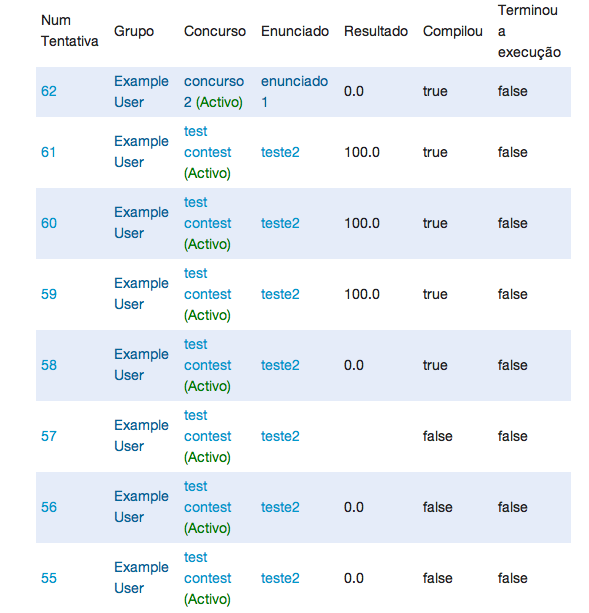
\includegraphics[scale=0.60]{Images/tentativas}
\caption{Página onde pode consultar as tentativas (vista das tentativas de todos os utilizadores)}\label{img:tentativas}
\end{center}
\end{figure}